\documentclass[11pt,a4paper]{article}
\usepackage[utf8]{inputenc}
\usepackage[T1]{fontenc}
\usepackage[margin=2.3cm]{geometry}
\usepackage{lmodern}
\usepackage{amsmath}
\usepackage{graphicx}
\usepackage{booktabs}
\usepackage{caption}
\usepackage{float}
\usepackage[hidelinks]{hyperref}
\graphicspath{{../../results/}}

\title{\textbf{Stock Price Forecasting with Deep Neural Networks:\\a Comparison of MLP, 1D-CNN, LSTM and GRU}}
\author{Diego Banfi\\[2pt]
\small M.Sc. in Telecommunications Engineering, University of L'Aquila\\
\small Course: Deep Neural Networks}
\date{}

\begin{document}
\maketitle

\begin{abstract}
\noindent This work compares four deep learning architectures for one-step-ahead forecasting of the daily closing price of Microsoft (MSFT) stock: a multilayer perceptron (MLP), a one-dimensional convolutional network (1D-CNN), a long short-term memory network (LSTM) and a gated recurrent unit network (GRU). The models are implemented in PyTorch and trained on twenty years of daily prices, using sliding windows of 29 days and a window-relative normalization that makes the problem scale-invariant. On the test period (February 2018 -- January 2021) the recurrent models perform best, and the GRU achieves the lowest error, with an RMSE of 3.17\% and an MAE of 2.33\% of the average price.
\end{abstract}

\section{Introduction}
Time series forecasting is a classic application of deep learning. Recurrent networks such as LSTM and GRU are designed to model temporal dependencies, while MLPs and convolutional networks treat a time window as a fixed-size input vector. The goal of this project is to compare these four families of models on the same dataset, with the same preprocessing and the same training procedure, and to evaluate them with standard regression metrics.

\section{Dataset}
The dataset contains 5{,}000 daily records of MSFT stock, from March 2001 to January 2021, with opening, high, low and closing prices and traded volume. There are no missing values. Only the closing price is used in this work. As shown in Figure~\ref{fig:price}, the price grows from about \$15 to about \$239 over the period, with a much faster growth in the last years.

\begin{figure}[H]
  \centering
  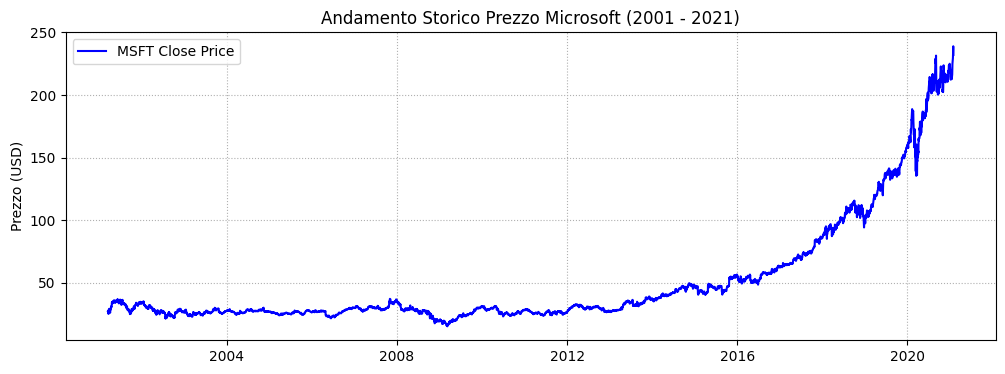
\includegraphics[width=0.85\textwidth]{msft_close_price_history.png}
  \caption{Historical closing price of MSFT stock (2001--2021).}
  \label{fig:price}
\end{figure}

\section{Method}

\subsection{Sliding windows and normalization}
The series is split into overlapping windows of $N = 30$ consecutive days: the first 29 days are the input and the 30th day is the target. Since the price range changes strongly over time, a global scaler fitted on the training years would produce test values far outside the training range. For this reason each window is divided by its first price $p_0$:
\begin{equation}
  \tilde{x}_k = \frac{p_k}{p_0}, \qquad k = 0, \dots, 29 .
\end{equation}
This window-relative normalization makes the problem scale-invariant and does not introduce data leakage, because $p_0$ is always a past value of the same window. Predictions are converted back to dollars by multiplying by $p_0$.

\subsection{Data split}
The 4{,}971 windows are split in chronological order, without shuffling between sets:
\begin{itemize}
  \item \textbf{training}: 70\% (targets up to February 2015);
  \item \textbf{validation}: 15\% (February 2015 -- February 2018);
  \item \textbf{test}: 15\% (February 2018 -- January 2021, 746 days).
\end{itemize}

\subsection{Architectures}
All models take as input a window of 29 normalized prices and output one value:
\begin{itemize}
  \item \textbf{MLP}: fully connected layers $29 \rightarrow 64 \rightarrow 32 \rightarrow 1$, ReLU activations and dropout 0.2.
  \item \textbf{1D-CNN}: 32 convolutional filters of size 3, max pooling of size 2, a dense layer of 32 neurons and the output layer.
  \item \textbf{LSTM}: one LSTM layer with 64 hidden units; the hidden state of the last time step is passed through dropout 0.2 and a dense layer of 32 neurons.
  \item \textbf{GRU}: same structure as the LSTM, with a GRU layer of 64 hidden units.
\end{itemize}

\subsection{Training}
All models are trained with the same procedure: MSE loss, Adam optimizer with learning rate $10^{-4}$, batch size 32, up to 30 epochs and early stopping with a patience of 10 epochs on the validation loss. The weights of the best validation epoch are restored at the end of training. Random seeds are fixed for reproducibility.

\subsection{Metrics}
The models are evaluated on the test set, in dollars, with the mean squared error (MSE), the root mean squared error (RMSE) and the mean absolute error (MAE). RMSE and MAE are also expressed as a percentage of the average test price (\$145.7).

\section{Results}
Table~\ref{tab:results} and Figure~\ref{fig:metrics} summarize the test results. Figure~\ref{fig:pred} compares the predictions with the real price over the whole test period and over the last 60 days.

\begin{table}[H]
  \centering
  \begin{tabular}{lccccc}
    \toprule
    \textbf{Model} & \textbf{RMSE [\$]} & \textbf{RMSE [\%]} & \textbf{MAE [\$]} & \textbf{MAE [\%]} & \textbf{MSE [\$$^2$]} \\
    \midrule
    \textbf{GRU}  & \textbf{4.61} & \textbf{3.17} & \textbf{3.40} & \textbf{2.33} & \textbf{21.28} \\
    LSTM          & 5.90 & 4.05 & 4.05 & 2.78 & 34.78 \\
    1D-CNN        & 6.14 & 4.21 & 4.14 & 2.84 & 37.65 \\
    MLP           & 6.89 & 4.73 & 4.72 & 3.24 & 47.46 \\
    \bottomrule
  \end{tabular}
  \caption{Test set metrics, sorted by RMSE.}
  \label{tab:results}
\end{table}

\begin{figure}[H]
  \centering
  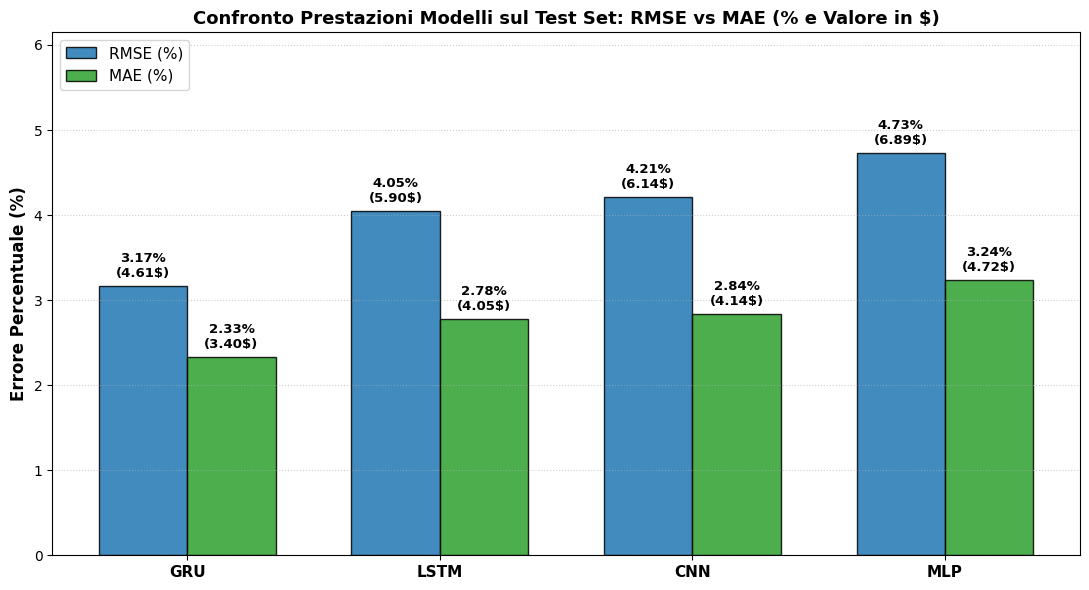
\includegraphics[width=0.8\textwidth]{metrics_comparison.png}
  \caption{RMSE and MAE of the four models on the test set.}
  \label{fig:metrics}
\end{figure}

\begin{figure}[H]
  \centering
  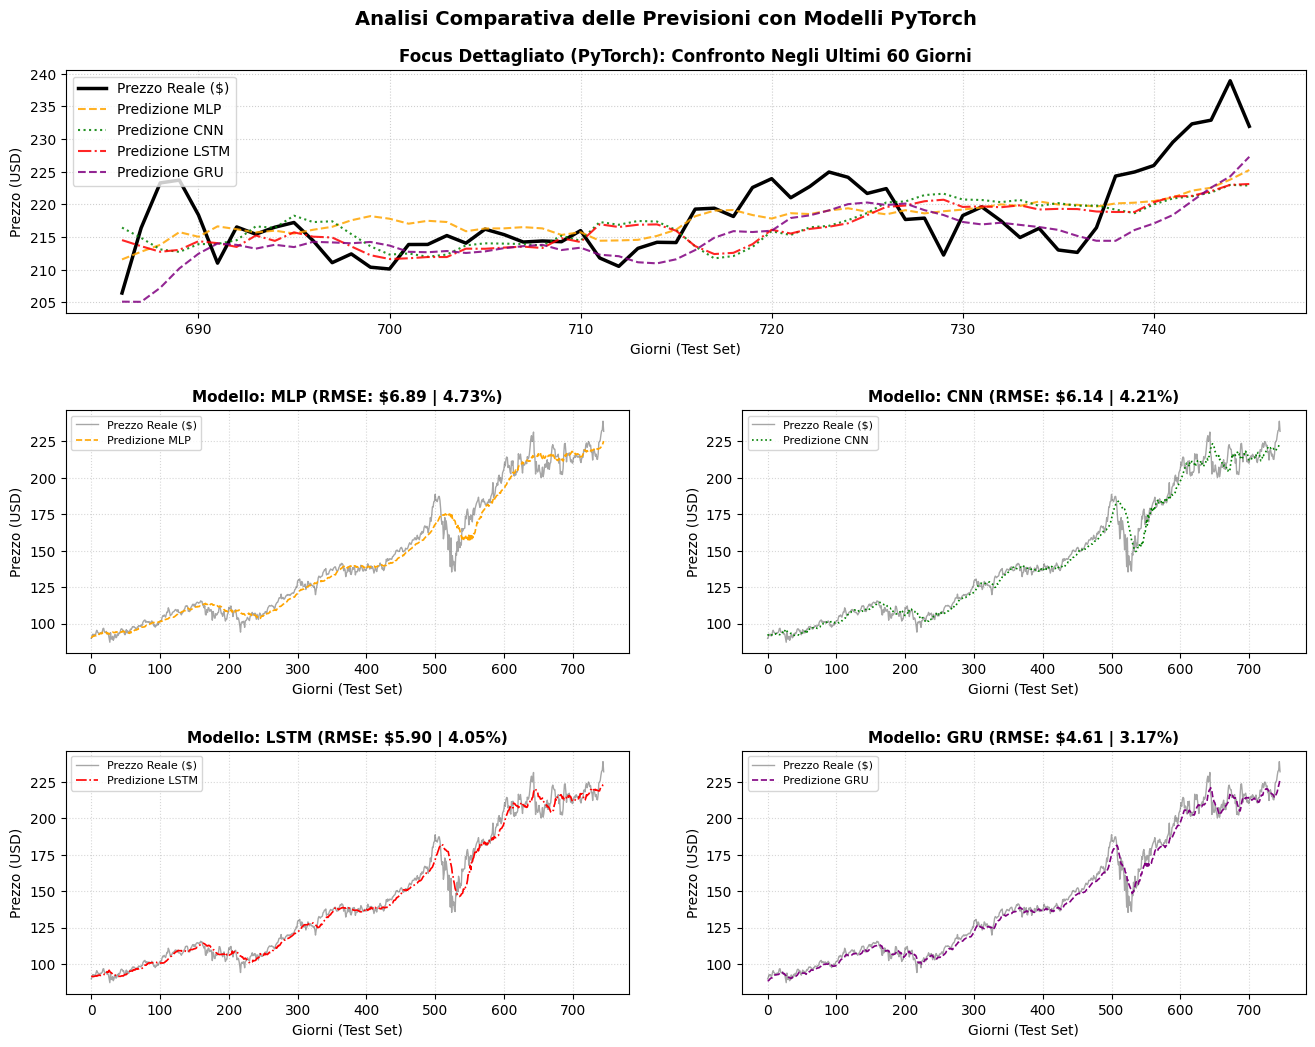
\includegraphics[width=0.95\textwidth]{predictions_comparison.png}
  \caption{Predicted and real closing price: last 60 days of the test set (top) and whole test set for each model.}
  \label{fig:pred}
\end{figure}

Figure~\ref{fig:loss} shows the training and validation loss of the GRU. The validation loss decreases together with the training loss, and early stopping selects the best epoch, which limits overfitting.

\begin{figure}[H]
  \centering
  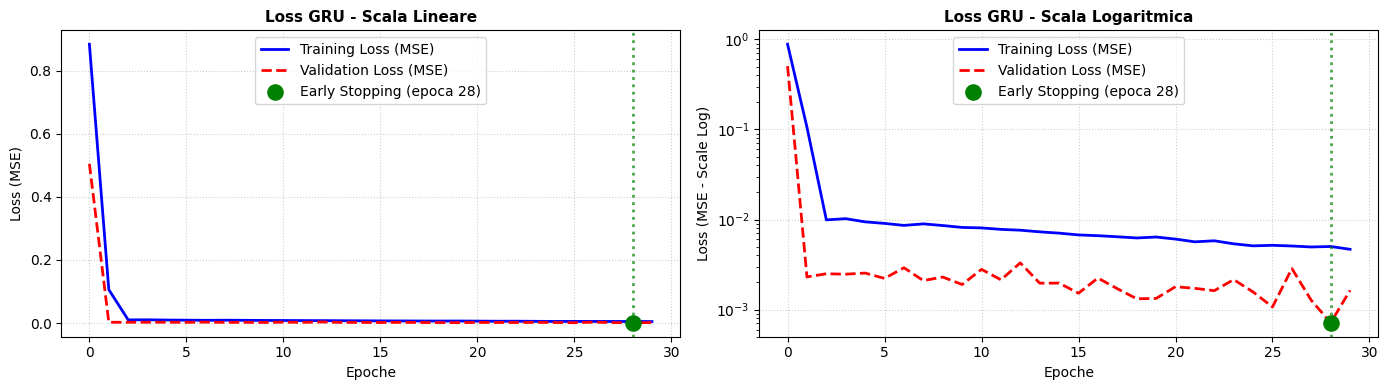
\includegraphics[width=0.95\textwidth]{gru_loss_and_prediction.png}
  \caption{Training and validation loss of the GRU, in linear and logarithmic scale.}
  \label{fig:loss}
\end{figure}

\section{Discussion}
\begin{itemize}
  \item \textbf{Recurrent models perform best.} GRU and LSTM process the window step by step and keep a memory of the previous days, which suits the sequential nature of the data. The GRU, with fewer parameters than the LSTM, gives the lowest error on this dataset.
  \item \textbf{1D-CNN and MLP} treat the window as a fixed input vector. The CNN captures local patterns and outperforms the MLP, but both follow fast changes of the price less closely, for example during the sharp drop of early 2020.
  \item \textbf{Normalization.} Window-relative normalization was essential: it allows models trained on prices of \$15--\$40 to predict prices above \$200 in the test period.
  \item \textbf{Limitations.} A naive persistence model, which predicts that tomorrow's price equals today's price, reaches an RMSE of 2.16\% on the same test set. This is a well-known property of daily stock prices, which behave almost like a random walk: the networks learn the overall trend, but do not yet extract information beyond the last observed price. Using additional inputs (volume, high and low prices, technical indicators) or predicting returns instead of prices are natural next steps.
\end{itemize}

\section{Conclusions}
Four deep learning architectures were compared on the same forecasting task with the same preprocessing and training. Recurrent networks gave the best results, and the GRU reached the lowest error (RMSE 3.17\%, MAE 2.33\%). The comparison with a naive persistence baseline shows that forecasting daily stock prices remains a hard problem, and suggests richer inputs and return-based targets as future work.

\end{document}
